\ssection{Architectural Write Latency Investigation}
In this section, we present the key architectural features and write latency behaviors that enable BREW-RC. 
By applying carefully selected test patterns to commercial ReRAM memories and analyzing the corresponding write latency, the memory array word size, polarity serialization properties, and timing perturbations due to embedded ECC functions can be observed. 
The results inform our subsequent ECC reverse engineering.
% These capabilities are exploited in the next section to recover the complete ECC function from each target memory.

\ssubsection{Experimental Setup}
The experiments in this paper are performed on four samples of two ReRAM products from RAMXeed (formerly Fujitsu Semiconductor Memory Solutions Ltd.), listed in Table \ref{tab:reram_spec}.
Each experiment collects write latencies, $t_w$ from a set of applied test vectors.
% \begin{equation}
% \mathcal{D} = \left(d_0^{(i)}, d_1^{(i)}, t_w^{(i)} \right)
% \end{equation}
% where $t_w^{(i)}$ is the measured write latency for the $i^{th}$ write operation transitioning an $n$-bit logically contiguous region from an initial state $d_0^{(i)} \in \left\{ 0,1\right\}^n$ to a final state
% $d_1^{(i)} \in \left\{ 0,1\right\}^n$.

Each write is committed to the device over a SPI interface by de-asserting chip-select following the last byte of a $\texttt{WRITE}$ operation. $t_w$ is measured from time the write transaction is committed, to the time the write-in-progress (WIP) bit of the STATUS register is cleared. Measurements of $t_w$ are quantized by the time required to check for the completion of a write ($\Delta t$). 
% Therefore, each write latency measurement is defined as
% \begin{equation}
% t_w \in \left\{i \Delta t \mid i \in \mathbb{N} \right\}
% \end{equation}
% where $i$ is the number of checks performed before for the $i^{th}$ write operation completes. 
$\Delta t$ is the minimum time required to perform a read status register (RDSR) operation on each RAMXeed module. The RDSR can be polled by continuing to drive the SPI clock after an initial opcode, returning the status after every 8 SPI cycles.
% The RDSR operation is required to determine when a committed write to memory completes. To perform a RDSR operation, the SPI bus must drive an initial 8-bit opcode followed by at least 8 SPI clock cycles to return the 8-bit status. After obtaining the first status byte, RDSR can continue to be polled by holding chip select while driving SPI clocks. In this polling mode, the status is returned every 8 SPI clock cycles (ignoring the initial opcode). 
The write completes when the write-in-progress (WIP) bit of the status register is cleared.

The sampling period for measurements of $t_w$ is defined as the time between successive RDSR operations: $\Delta t = {8}/{f_{SPI}}.$
We operate the SPI interfaces at the maximum frequency defined in the specification. Therefore, the minimum $\Delta t$ of the MB85AS4MT and MB85AS8MT memories are 1.6$\mu$s and 0.8$\mu$s, respectively.
%For any measurement of $t_w$, $\hat{t_w}$,  $t_w$ is at most $\hat{t_w}$ and at least $\hat{t_w} + T_{sample}$. In the write latency distributions presented in the rest of the paper, each measured $t_w$ is therefore quantized as
% \begin{equation}
% t_{k-1} \; T_{sample} < t_w \le t_k \; T_{sample} \implies \widehat{t}_w=t_k
% \end{equation}

We apply and time SPI transactions using a Terasic DE10-Nano Cyclone V SoC FPGA development kit. For each write operation, a counter on the FPGA captures $t_w$, which is then pushed to a response FIFO. The FPGA is used primarily to scale our experiments to many chips. Prior works have demonstrated similar timing capabilities using microcontrollers \cite{tolga2024trng, ferdaus2024hiding}.

\begin{table}[t!]
	\centering
	\caption{RAMXeed ReRAM device comparison.}
	\label{tab:reram_spec}
	\renewcommand{\arraystretch}{1.0}
	\setlength{\tabcolsep}{3.5pt}
	\begin{minipage}{0.98\columnwidth}
		\centering
		\begin{tabular}{lcccc}
			\toprule
			\textbf{Device}    & \textbf{Capacity}  & \textbf{SPI} $\mathbf{f_{\max}}$ &
			\textbf{Endurance} & \textbf{Buf. Size}                                                              \\
			\midrule
			\textbf{MB85AS4MT} & 4\,Mb              & 5\,MHz                           & 1.2M\,Times/B  & 256\,B \\
			\textbf{MB85AS8MT} & 8\,Mb              & 10\,MHz                          & 1M\,Times/4\,B & 256\,B \\
			\bottomrule
		\end{tabular}
	\end{minipage}
	% \vspace{-.5cm}
\end{table}


\ssubsection{Investigation Results}
\label{sec:investigation-expts}
We first present a series of experiments performed on the devices in  Table \ref{tab:reram_spec}.
Measurements are carried out on 4 samples of each device.

\ssubsubsection{\textbf{Expt.~I Redundant Write, Write Latency}}
%\ssubsection*{Expt.~I Redundant Writes}
\label{sec:red}
\label{exp:i}

% \begin{algorithm}[b]
\footnotesize
\caption{redundant write test pattern generation \label{alg:red}}
\begin{algorithmic}[1]
\State $N_{\text{ADDRS}} \gets 10$
\State $A \gets$ rand\_256B\_aligned\_addrs($N_{\text{ADDRS}}$)
\ForAll{address \textbf{ in } $A$}
    \State $\mathrm{S} \gets$ get\_rand\_256B\_pattern() 
    \State $L \gets$ shuffle(range(1, 256))
    \State write\_$\mathrm{S}$(address, $\mathrm{S}$) \Comment{1, 256-byte write op}
    \ForAll{$i$ \textbf{ in } $L$}
        \State write\_bytes(address, $\mathrm{S}[0{:}i]$) 
        \Comment{1, $i$-byte write op}
    \EndFor
\EndFor
\end{algorithmic}
\end{algorithm}


In a crossbar-based architecture, the word size of the memory array is the smallest unit that can be serialized through the write path. The word size is the natural choice for the ECC encoder data word width ($k$). Our target memories allow 1-256B write operations. However, the physical word size of the target devices is not known.

To infer $k$, we use the latency characteristics of redundant write operations. A \textit{redundant write} reinforces the existing logical state of ReRAM cells. Because no transitions occur, the write latency reflects the minimum $t_{w}$ (Table \ref{tab:polarity-mix}) and the fixed per-word programming overhead of the controller. 
We perform redundant writes with burst sizes of 1-256B on 10 randomly selected 256B-aligned addresses. First, we program a 256B contiguous memory segment ($\mathrm{S}$) to a random initial state. Then, for each byte position $i_B$ within ($\mathrm{S}$), an $i_B$-byte redundant write is performed.

%This makes redundant writes a low noise probe of the write-path serialization granularity. 





Figure \ref{fig:red-scan} shows the combined write latencies (mean and shaded 95\% confidence interval) for all samples and test addresses. For each 4M (8M) sample, at all addresses, and across all randomly initialized $S$ states, $t_w$ overheads are accrued every two (four) byte-lengths and show almost no variance. This result demonstrates that 4M (8M) redundant write times do not show a clear data dependency, and that serialization occurs on 2B (4B) boundaries, indicating $k_{4M}=16$ bits ($k_{8M}=32$ bits). $k_{4M}$ and $k_{8M}$ provide one dimension of the $k\times r$ parity submatrix.
\begin{figure}[t!]
    \centering
    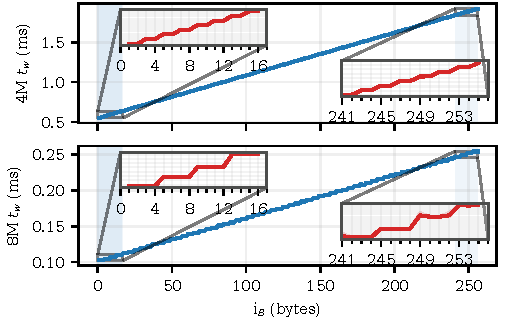
\includegraphics[width=0.95\linewidth]{fig/images/pdf/redundant-bytes-lineplots.pdf}
    \vspace{-.45cm}
    \caption{Write latency measurements ($t_w$) for $i$-byte redundant write operations on 4M (top) and 8M (bottom) devices.}
    % \vspace{-.65cm}
    % The aggregated redundant write times of four MB85AS4MT and four MB85AS8MT. All bursts are measured 10 times at 10 random 256B base addresses on each chip. All initial buffer data is randomized\, and each burst amount overwrites data redundantly from the base address up to the burst amount.}
    \label{fig:red-scan}
\end{figure}

\ssubsubsection{\textbf{Expt.~II 1-bit Transitions, Uniform $\mathrm{S}$}}
%\ssubsection*{Expt.~II Locally Uniform 1-bit Transitions}
\label{exp:ii}
In this experiment, we characterize single-bit write latency in uniformly-initialized 256-byte segments ($S$).
Single-bit transitions may exhibit data-dependent $t_w$ if there are asymmetries in the switching dynamics of the ReRAM cells and/or the PV loop.

% \begin{algorithm}[t]
\footnotesize
\caption{1-bit, uniform $\mathrm{S}$, test pattern generation \label{alg:1bit}}
\begin{algorithmic}[1]
\State $N_{\text{ADDRS}} \gets 10$
\State $A \gets$ rand\_256B\_aligned\_addrs($N_{\text{ADDRS}}$)
\ForAll{address \textbf{ in } $A$}
    \ForAll{$\mathrm{S}$ \textbf{ in } [$\mathbf{0}$, $\mathbf{1}$]}
        \State init\_$\mathrm{S}$(address, $\mathrm{S}$) \Comment{1, 256-byte write op}
        \State $L \gets$ shuffle(range(0, 2047))
        \ForAll{$i_{\text{b}}$ \textbf{ in } $L$}
            \State toggle\_bit\_i\_twice($\mathrm{S}$, $i_{\text{b}}$) 
            \Comment{2, 1-byte write ops}
        \EndFor
    \EndFor
\EndFor
\end{algorithmic}
\end{algorithm}



A 256-byte span ($\mathrm{S}$) is initialized to $\mathrm{S}=\mathbf{0}$ (all zeros)  or $\mathrm{S}=\mathbf{1}$  (all ones). Each bit positions ($i_b$) in the 2048-bit span is toggled 10 times and write latencies are captured. Since the minimum write size in both memories is 1 byte, we calculate the byte-offset and target data bit from $i_b$ and perform two 1-byte write latency measurements, toggling bit $i_b$ in both logical polarities.


Figure~\ref{fig:1b-buff-scan} demonstrates $t_w$ distributions for each chip.
Each bar in Figure~\ref{fig:1b-buff-scan} represents a log-scaled collapsed histogram, combining all bit positions and experiment addresses for one polarity, initial uniform state, and chip. 
Because the distributions are long-tailed, we truncate the plot at the 95th percentile to improve visibility.

The measured write latency distributions for each polarity measured from the 4M subtly overlap but are distinguishable. For the 8M, write latency distributions for each polarity are separated by a large margin. These write latency polarity relationships are preserved across all MB85AS4MT and MB85AS8MT samples. This experiment demonstrates that single-bit transitions of each memory produce data dependent write latency distributions.

\begin{figure}[h!]
    \centering
    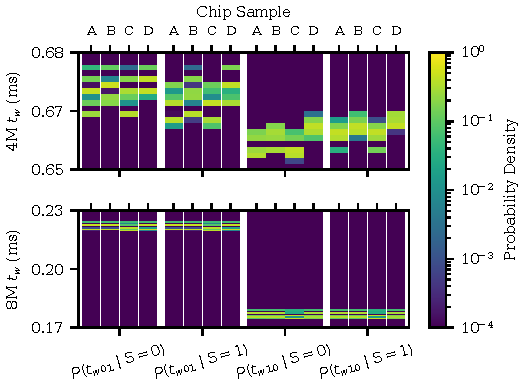
\includegraphics[width=0.95\linewidth]{fig/images/pdf/single-bit-buffer-scans-heat-bars.pdf}
    \vspace{-.5cm}
    \caption{Write latency distributions for 1-bit transitions within uniformly initialized 256-byte segments measured on 4 4M samples (top) and 4 8M samples (bottom). Each heatmap bar is a collapsed histogram colored according to the log-probability of observing a $t_w$ in each $\Delta t$-sized bin. $t_{w01}$ and $t_{w10}$ latencies correspond to data word transitions with a DHD of $\left(1,0 \right)$ and $\left(0,1\right)$, respectively. \label{fig:1b-buff-scan}}
\end{figure}
\begin{figure}[!h]
    \centering
    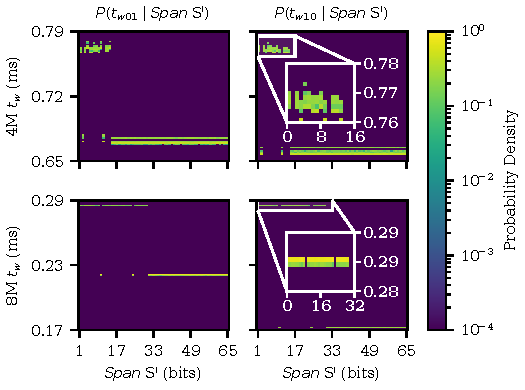
\includegraphics[width=0.95\linewidth]{fig/images/pdf/single-bit-sensitivity-scans-heat-bars-inset.pdf}
    \vspace{-.4cm}
    \caption{Write latency distributions for 1-bit $t_{w01}$ (left) and $t_{w10}$ (right) transitions within non-uniformly initialized 256-byte segments. Measurements from all 4 4M samples (top) and 4 8M samples (bottom) are aggregated. Each heatmap bar is a collapsed histogram colored according to the log-probability of observing a $t_w$ in each $\Delta t$-sized bin. The right plots zoom into the upper $t_w$ distributions to show 1-bit transitions that become \texttt{BIPOLAR} due to parity bit activity. \label{fig:sensitivity-scan}}
\end{figure}

\ssubsubsection{\textbf{Expt.~III 1-bit Transitions, Nonuniform $\mathrm{S}$}}
% \ssubsection*{Expt.~III Locally non-uniform 1-bit transitions}
\label{exp:iii}

% \begin{algorithm}[b!]
\footnotesize
\caption{1-bit, non-uniform $\mathrm{S}$, test pattern generation \label{alg:sensitivity}}
\begin{algorithmic}[1]
\State $N_{\text{ADDRS}} \gets 10$
\State $A \gets$ rand\_sample(align\_256B(addresses), $N_{\text{ADDRS}}$)
\State $\mathrm{S} \gets \mathbf{0}$
\ForAll{address \textbf{ in } $A$}
    \State $L \gets$ shuffle(range(1, 2047))
    \ForAll{$s$ \textbf{ in } $L$}
        \State $\mathrm{S}' \gets$ initialize\_$\mathrm{S}'$($\mathrm{S}$, $s$) \Comment{1, 256-byte write op}
        \State toggle\_bit\_0\_twice($\mathrm{S}'$) \Comment{2, 1-byte write ops}
    \EndFor
\EndFor
\end{algorithmic}
\end{algorithm}

ECC parity bit transition polarities depend on the state of a data word ($d$). In this experiment, we demonstrate that the state of non-transitioning bits can influence the $t_w$ distribution, indicating the presence of parity bits. By making $S$ non-uniform in the same word boundary as a transitioning bit, we demonstrate three distinct latency distributions. 
%In the next experiment, we demonstrate that these distributions correspond to the $\texttt{UNIPOLAR}_N$, $\texttt{UNIPOLAR}_P$, and \texttt{BIPOLAR} transitions in Table \ref{tab:polarity-mix}.

We randomly select 10 256-byte-aligned addresses. From each address, a 256-byte segment is initialized to all zeros ($\mathrm{S}=\mathbf{0}$).  
The first bit in each segment is designated as the \emph{measurement bit}.  
Before each measurement sequence, a contiguous subset of neighboring bits extending from the measurement bit is inverted ($\mathrm{S}[1:i] = \mathrm{S}' = \mathbf{1}$), creating a locally non-uniform initial state.  
Each measurement bit is toggled 10 times per configuration, with $\mathrm{S}'$ span sizes ($i$) ranging from 1 to 2047 bits.



The resulting distributions are shown in Figure~\ref{fig:sensitivity-scan}, with $\mathrm{S}'$ span sizes from 1-64. We make two key observations. First, beyond the word size reported in \hyperref[exp:i]{Exp.~I}, the distribution of write times stabilizes.
That is, the influence of nearby bit-states on write latency ends at the logical word boundary.  
Once the $\mathrm{S}'$ span exceeds the word length ($k$), the measured write latency distribution is identical to our prior, uniform $\mathrm{S}$, experiment.
Second, while the span of $\mathrm{S}'$ is smaller than the word boundary, single-bit writes generally exhibit longer latencies than those observed in uniform segments.
%In Section~\ref{}, we demonstrate that these high latency distributions are identical to those occupied by bipolar transitions.

% This effect is observed for both write polarities, and can be explained by non-uniform data causing parity bit activity in the opposing polarity to the measurement bit.  
% However, in both the MB85AS4MT and MB85AS8MT, two specific $\mathrm{S}'$ span configurations yield latency distributions nearly identical to those of the uniform baseline. These anomalies can be explained as data word configurations that result in consistent data and parity bit transition polarities.

% In summary, 1-bit write transitions demonstrate that the write polarity can be identified from uniformly initialized word boundaries. Additionally, the latency of 1-bit transitions is sensitive to the logical state of other bits within the same word. In the next experiment, we demonstrate that the highest write-latency cluster observed in \hyperref[exp:iii]{Exp. III} is the same latency cluster observed when measuring multi-bit bipolar byte transitions.

\ssubsubsection{\textbf{Expt.~IV 1-byte Transitions, Uniform $S$}}
\label{sec:1byte}
\label{exp:iv}
% We now characterize $t_w$ for all single-byte transitions on the MB85AS4MT and MB85AS8MT devices. The purpose of the following experiment is to identify the write latency properties of multi-bit transitions occurring within word boundaries. From our results, we are able to link $t_w$ timing cluster membership to unipolar and bipolar transitions.
% \paragraph*{\textbf{Exp.~IV 1-byte transitions}} 
In this experiment, we measure $t_w$ for all possible ($2^{16}$) single-byte transitions for all 4M and 8M samples.
This experiment is similar to the 1-byte latency characterization performed in \cite{tolga2024trng} where the 4M device was evaluated as an entropy source for true random number generators (TRNGs). We repeat the same experiment here. For each chip, the experiment is performed on 10 word-sized segments. We vary the state of all inactive bytes in the word, setting them to either all 1's or all 0's, and repeat our measurements for all bytes within each target segment. For each chip, to suppress the effect or rare long-tailed latency measurements, we take the minimum $t_w$ ($t_{wmin}$) for each byte transition across all segments.

Figure \ref{fig:sierp-hist} shows the results of this experiment for the 4M and 8M. We observe 3 unique $t_w$ distributions for the 4M chip, and 4 for the 8M chip. The minimum $t_w$ measurement distribution is exclusively occupied by redundant write operations. Bipolar dataword transitions always occupy the highest $t_w$ distribution. Unipolar dataword transitions occupy either a intermediate $t_w$ distribution or the highest $t_w$ distribution. For the 4M, unipolar dataword transitions occupying the intermediate $t_w$ distribution overlap. For the 8M, there are two distinct intermediate $t_w$ distributions, each occupied by $t_w$ measurements of a single datword transition polarity. These timing observations are consistent with \cite{tolga2024trng}. Our observation that certain \texttt{UNIPOLAR} transitions occupy \texttt{BIPOLAR} timing distributions suggests that underlying parity bit activity impacts the DHD of the write, causing polarity serialization.

% Considering the word boundaries identified Section \ref{sec:prelim-expts}, we expand this experiment to include all 2 (4) byte positions for each 2-byte (4-byte) word boundary within the MB85AS4MT (MB85AS8MT).
% \paragraph*{\textbf{Exp.~IV 1-byte transitions within 1-word writes}} 
% For each chip, we measure all byte transition $t_w$ for all byte positions of 10 word-sized segments ($\mathrm{S}$) where each word is initialized to either $\mathrm{S}=\mathbf{1}$ or $\mathrm{S}=\mathbf{0}$. Because our $t_w$ distributions are asymmetric and contain rare extreme-latency measurements, we use the per-chip minimum across all segments for each byte index and transition. This allows us to ensure these measurements do not impair our ability to distinguish the appropriate write latency distribution for each $t_w$.
% Test patterns are generated using Algorithm \ref{alg:1byte}. 
% We observe the same Sierpinski pattern as \cite{tolga2024trng} when our 4M measurements are visualized as a heatmap. We show our results as a histogram so that we can describe data-dependent polarity relationships for both the 4M and 8M in greater detail. 

% We assume that our $t_w$ measurement distributions map to the transition behavior of full codewords. In this context, parity bit activity cannot force a bipolar data word transition to produce a unipolar $t_w$, but it can cause a unipolar data word transition to occupy a bipolar $t_w$ if any parity bits transition toward an opposing polarity. If parity bits do not toggle or toggle only in a direction consistent with the applied data word transition, then the parity bits have no effect on the distribution that the resulting $t_w$ occupies. We identify each $t_{wmin}$ distribution using a parametric mixture model and label each mixture component shown in Figure \ref{fig:sierp-hist} with our inferred codeword behavior.

% The two initial states are used to confirm our prior finding that the state of the other bytes in the word effect the latencies of each byte under test. We note that similar analyses and visualization techniques as we present below have been performed on the MB85AS4MT device in \cite{tolga2024trng}, although this investigation did not consider the state of the other bytes in the word.
% To capture all 1-byte transition times we generate test patterns using Algorithm \ref{alg:1byte}. 
% % Note that each byte-transition is performed by writing an entire word. 
% % We choose to commit an entire word (where only 1 byte is active) for post-processing convenience and to maintain a similar data pattern between this experiment and the final one used for our SAT constraint encoding in Section \ref{sec:sat-encoding}.
% % \FloatBarrier
% \begin{algorithm}[!t]
\footnotesize
\caption{1-byte test pattern generation \label{alg:1byte}}
\begin{algorithmic}[1]
\State $B \gets$ word\_bytes() \Comment{2 for 4Mb, 4 for 8Mb}
\State $N_{\text{WORDS}} \gets 10$
\State $W \gets$ rand\_word\_aligned\_addrs($B$, $N_{\text{WORDS}}$)
\ForAll{word\_addr \textbf{ in } $W$}
    \ForAll{$G$ \textbf{ in } [$\mathbf{0}$, $\mathbf{1}$]}
        \State init\_word(word\_addr, $G$) \Comment{1, $B$-byte write op}
        \State $P \gets$ shuffle(range(0, $B{-}1$))
        \ForAll{byte\_pos \textbf{in} $P$}
            \State $Tr \gets$ get\_all\_byte\_transitions\_rand\_order()
            % \State from\_byte $\gets$ pack\_byte(byte\_pos, Tr[0].from)
            \State from\_byte $\gets$ Tr[0].from
            \State write\_byte(word\_addr, from\_byte)
            \Comment{1, 1-byte write op}
            \ForAll{tr \textbf{in} $Tr$}
                \State to\_byte $\gets$ tr.to
                \State write\_byte(word\_addr, to\_byte)
                \Comment{1, 1-byte write op}
            \EndFor
        \EndFor
    \EndFor
\EndFor
\end{algorithmic}
\end{algorithm}

\begin{figure}[t!]
    \centering
    \hspace{-0.75cm}
    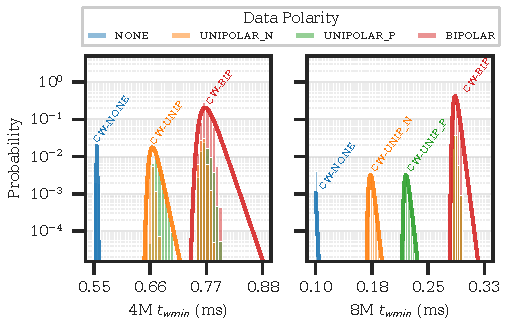
\includegraphics[width=0.95\columnwidth]{fig/images/pdf/sierpinski-clustering-mixture-curves.pdf}
    \vspace{-.45cm}
    \caption{4Mb and 8Mb $t_{wmin}$ measured for all 1-byte transitions. Histogram bars are colored according to data polarity. The curves correspond to EM-fitted mixture components that trace our observed latency clusters. We label each component according to our inferred codeword behavior \label{fig:sierp-hist}.}
    % \vspace{-.65cm}
\end{figure}
% % \FloatBarrier
% The results of our single-byte experiments are shown to the right in Figure \ref{fig:1B-sierpinski-scan}. We represent all transition times as pixels in a heatmap. For each heatmap, the x-axis is the initial state (FROM byte) of the transitioning byte in the word and the y-axis is it's final state (TO byte). 
% For this experiment, we take the minima of each per-chip write-latency distribution for each (TO, FROM) pair ($\min\left(t_{w}\right)$), to ensure long-tail write latencies do not bias aggregate statistics. We then average $\min\left(t_{w}\right)$ across all samples of each memory. We include two byte positions for each global setting. 

% As first identified in \cite{tolga2024trng}, a Sierpinski-like relationship with a minor hamming weight bias exists between all 1-byte transition test patterns and measured write latency. On the left of Figure \ref{fig:1B-sierpinski-scan}, a reference Sierpinski gasket is shown with a hamming weight bias. This image is generated by coloring points in the transition map where unipolar byte transitions occur. We also apply a small bias scaled to the total hamming weight of each transition to produce a close approximation of the measured heatmaps. Our measurements show three significant timing clusters (colors) for each heatmap. The fastest write latency group (black), always corresponds to redundant 1-byte write operations. The second fastest group (teal/blue) always corresponds 1-byte write operations with unipolar transitions. However, the slowest timing group (green/yellow) contains 1-byte write operations with both unipolar and bipolar transitions, puncturing the perfect Sierpinski gasket. Here we define a \textit{puncture} as a unipolar data-word transition whose write latency is similar to bipolar data word transitions. 

% Both bipolar and \emph{punctured} unipolar writes result in a similar $t_w$ as the long 1-bit writes observed under non-uniform initialization in the prior experiment.

% These results are consistent with the presence of a latent function that forces seemingly unipolar transitions (e.g. 1-bit transitions, unipolar byte transitions) to produce a bipolar write latency behavior. Within a crossbar memory, ECC is the most likely cause of this behavior. ECC parity bit states depend on the state of the data word. As parity bits are generally produced by XOR functions, when all but one bit in a data word is zero the transitioning bit is passed through. 

% In this case, if the parity matrix (P) produces parity bit transitioning in a direction oposing unipolar write data, this contradiction is expected.
% % out prior result where distribution shifts were observed for single-bit transitions, where the state of other bits in the word were changed ahead of transition measurements. 
% % From our \hyperref[exp:2ii]{Exp.~III} results, we found that there is a coupling between word-level bit states and write transition time. This results of this experiment demonstrates that the same coupling influences multi-bit transitions and that the timing cluster assignment of each transition is, for the most part, polarity dependent, and only violated when a unipolar data word results in bipolar timing. This effect suggests the presence of an ECC in our target memories. 
% As described in Section \ref{sec:bg}, ECC parity functions couple data bits to parity bits which are encoded and written in parallel with data bits. If parity bits update in a polarity opposing a unipolar data word transition, then the effective polarity (i.e. the polarity of the codeword transition) becomes bipolar. If they do not, then the entire codeword has a consistent polarity and the transition is unipolar. Bipolar transitions remain bipolar, independent of parity bit updates. This behavior perfectly describes our observations above. However, without the exact parity matrix, we cannot predict where parity bit perturbations will cause write latencies to diverge from the expected. In the next section we describe how BREW-RC capitalizes on this timing relationship to extract a bit-exact parity matrix from timing-polarity relationships.

\label{sec:clustering}
